\section{How do we produce sound?}
Our voice is also produced by vibrations.

\section{Activity: Feeling the Vibrations in Your Throat}
\subsection{Procedure}
Place your fingers gently on the front of your throat. Say ``Aaa..." loudly for a few seconds. Repeat the activity while whispering ``Aaa...". Compare what you feel in both cases.

\newthought{Observe} Do you feel vibrations in your throat when you speak? Do you feel the same vibrations when you whisper?

\newthought{Discussion} Inside your throat is a small organ called the voice box or larynx. It contains two small muscular bands called vocal cords.
\begin{marginfigure}
  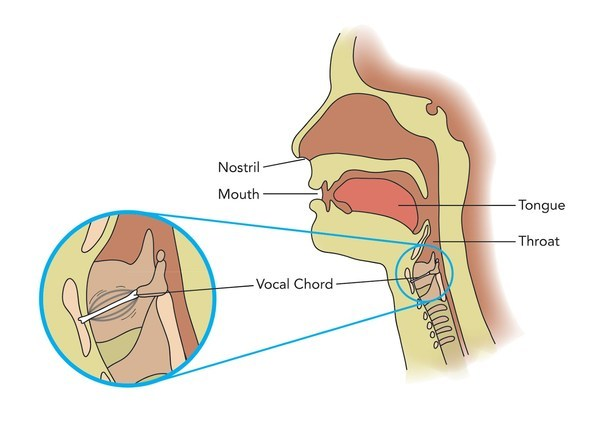
\includegraphics{vocalcord}
  \caption{Our vocal chords vibrate when we produce sound. Image source: SASOL Inzalo Foundation}
\end{marginfigure}
When you breathe, air passes freely through the voice box. When you speak or sing, the vocal cords come close together. Air from the lungs passes between them and makes them vibrate rapidly. These vibrations produce sound.

When you whisper, the vocal cords do not vibrate in the same way. That is why you do not feel the same vibrations in your throat.

\subsection{How Do We Form Different Sounds?}

The sound produced by the vocal cords is only a basic buzzing sound. This sound is shaped into speech by different parts of our mouth. Our tongue, lips, teeth, the roof of the mouth (palate), and the nose work together to produce different sounds and words.

\begin{fullwidth}
\begin{table}[h]
  \centering
  \begin{tabular}{ll}
        \toprule
        Letter & How the sound is made with your mouth, nose, and tongue?\\ 
        \midrule
        {\tam ப} (pa) &Close both lips tightly, then open them suddenly\\
        {\tam ம} (ma) & Close both lips. Let the sound come out through your nose\\
        {\tam த} (tha)& Touch the tip of your tongue to your upper front teeth.\\
        {\tam ல} (la) & Touch the tip of your tongue to the bumpy part just behind your upper front teeth.\\
        {\tam ள} (la) & Curl the tip of your tongue slightly backwards and touch the roof of your mouth.\\
        {\tam ழ} (zha) & Curl the tip of your tongue slightly backwards, but do not let it touch the roof of your mouth.\\
        \bottomrule
  \end{tabular}
\end{table}
\end{fullwidth}